\documentclass[]{book}
\usepackage{lmodern}
\usepackage{amssymb,amsmath}
\usepackage{ifxetex,ifluatex}
\usepackage{fixltx2e} % provides \textsubscript
\ifnum 0\ifxetex 1\fi\ifluatex 1\fi=0 % if pdftex
  \usepackage[T1]{fontenc}
  \usepackage[utf8]{inputenc}
\else % if luatex or xelatex
  \ifxetex
    \usepackage{mathspec}
  \else
    \usepackage{fontspec}
  \fi
  \defaultfontfeatures{Ligatures=TeX,Scale=MatchLowercase}
\fi
% use upquote if available, for straight quotes in verbatim environments
\IfFileExists{upquote.sty}{\usepackage{upquote}}{}
% use microtype if available
\IfFileExists{microtype.sty}{%
\usepackage{microtype}
\UseMicrotypeSet[protrusion]{basicmath} % disable protrusion for tt fonts
}{}
\usepackage[margin=1in]{geometry}
\usepackage{hyperref}
\hypersetup{unicode=true,
            pdftitle={Data Science for Physicians (DS4P)},
            pdfauthor={Peter Higgins},
            pdfborder={0 0 0},
            breaklinks=true}
\urlstyle{same}  % don't use monospace font for urls
\usepackage{natbib}
\bibliographystyle{apalike}
\usepackage{color}
\usepackage{fancyvrb}
\newcommand{\VerbBar}{|}
\newcommand{\VERB}{\Verb[commandchars=\\\{\}]}
\DefineVerbatimEnvironment{Highlighting}{Verbatim}{commandchars=\\\{\}}
% Add ',fontsize=\small' for more characters per line
\usepackage{framed}
\definecolor{shadecolor}{RGB}{248,248,248}
\newenvironment{Shaded}{\begin{snugshade}}{\end{snugshade}}
\newcommand{\AlertTok}[1]{\textcolor[rgb]{0.94,0.16,0.16}{#1}}
\newcommand{\AnnotationTok}[1]{\textcolor[rgb]{0.56,0.35,0.01}{\textbf{\textit{#1}}}}
\newcommand{\AttributeTok}[1]{\textcolor[rgb]{0.77,0.63,0.00}{#1}}
\newcommand{\BaseNTok}[1]{\textcolor[rgb]{0.00,0.00,0.81}{#1}}
\newcommand{\BuiltInTok}[1]{#1}
\newcommand{\CharTok}[1]{\textcolor[rgb]{0.31,0.60,0.02}{#1}}
\newcommand{\CommentTok}[1]{\textcolor[rgb]{0.56,0.35,0.01}{\textit{#1}}}
\newcommand{\CommentVarTok}[1]{\textcolor[rgb]{0.56,0.35,0.01}{\textbf{\textit{#1}}}}
\newcommand{\ConstantTok}[1]{\textcolor[rgb]{0.00,0.00,0.00}{#1}}
\newcommand{\ControlFlowTok}[1]{\textcolor[rgb]{0.13,0.29,0.53}{\textbf{#1}}}
\newcommand{\DataTypeTok}[1]{\textcolor[rgb]{0.13,0.29,0.53}{#1}}
\newcommand{\DecValTok}[1]{\textcolor[rgb]{0.00,0.00,0.81}{#1}}
\newcommand{\DocumentationTok}[1]{\textcolor[rgb]{0.56,0.35,0.01}{\textbf{\textit{#1}}}}
\newcommand{\ErrorTok}[1]{\textcolor[rgb]{0.64,0.00,0.00}{\textbf{#1}}}
\newcommand{\ExtensionTok}[1]{#1}
\newcommand{\FloatTok}[1]{\textcolor[rgb]{0.00,0.00,0.81}{#1}}
\newcommand{\FunctionTok}[1]{\textcolor[rgb]{0.00,0.00,0.00}{#1}}
\newcommand{\ImportTok}[1]{#1}
\newcommand{\InformationTok}[1]{\textcolor[rgb]{0.56,0.35,0.01}{\textbf{\textit{#1}}}}
\newcommand{\KeywordTok}[1]{\textcolor[rgb]{0.13,0.29,0.53}{\textbf{#1}}}
\newcommand{\NormalTok}[1]{#1}
\newcommand{\OperatorTok}[1]{\textcolor[rgb]{0.81,0.36,0.00}{\textbf{#1}}}
\newcommand{\OtherTok}[1]{\textcolor[rgb]{0.56,0.35,0.01}{#1}}
\newcommand{\PreprocessorTok}[1]{\textcolor[rgb]{0.56,0.35,0.01}{\textit{#1}}}
\newcommand{\RegionMarkerTok}[1]{#1}
\newcommand{\SpecialCharTok}[1]{\textcolor[rgb]{0.00,0.00,0.00}{#1}}
\newcommand{\SpecialStringTok}[1]{\textcolor[rgb]{0.31,0.60,0.02}{#1}}
\newcommand{\StringTok}[1]{\textcolor[rgb]{0.31,0.60,0.02}{#1}}
\newcommand{\VariableTok}[1]{\textcolor[rgb]{0.00,0.00,0.00}{#1}}
\newcommand{\VerbatimStringTok}[1]{\textcolor[rgb]{0.31,0.60,0.02}{#1}}
\newcommand{\WarningTok}[1]{\textcolor[rgb]{0.56,0.35,0.01}{\textbf{\textit{#1}}}}
\usepackage{longtable,booktabs}
\usepackage{graphicx,grffile}
\makeatletter
\def\maxwidth{\ifdim\Gin@nat@width>\linewidth\linewidth\else\Gin@nat@width\fi}
\def\maxheight{\ifdim\Gin@nat@height>\textheight\textheight\else\Gin@nat@height\fi}
\makeatother
% Scale images if necessary, so that they will not overflow the page
% margins by default, and it is still possible to overwrite the defaults
% using explicit options in \includegraphics[width, height, ...]{}
\setkeys{Gin}{width=\maxwidth,height=\maxheight,keepaspectratio}
\IfFileExists{parskip.sty}{%
\usepackage{parskip}
}{% else
\setlength{\parindent}{0pt}
\setlength{\parskip}{6pt plus 2pt minus 1pt}
}
\setlength{\emergencystretch}{3em}  % prevent overfull lines
\providecommand{\tightlist}{%
  \setlength{\itemsep}{0pt}\setlength{\parskip}{0pt}}
\setcounter{secnumdepth}{5}
% Redefines (sub)paragraphs to behave more like sections
\ifx\paragraph\undefined\else
\let\oldparagraph\paragraph
\renewcommand{\paragraph}[1]{\oldparagraph{#1}\mbox{}}
\fi
\ifx\subparagraph\undefined\else
\let\oldsubparagraph\subparagraph
\renewcommand{\subparagraph}[1]{\oldsubparagraph{#1}\mbox{}}
\fi

%%% Use protect on footnotes to avoid problems with footnotes in titles
\let\rmarkdownfootnote\footnote%
\def\footnote{\protect\rmarkdownfootnote}

%%% Change title format to be more compact
\usepackage{titling}

% Create subtitle command for use in maketitle
\newcommand{\subtitle}[1]{
  \posttitle{
    \begin{center}\large#1\end{center}
    }
}

\setlength{\droptitle}{-2em}
  \title{Data Science for Physicians (DS4P)}
  \pretitle{\vspace{\droptitle}\centering\huge}
  \posttitle{\par}
  \author{Peter Higgins}
  \preauthor{\centering\large\emph}
  \postauthor{\par}
  \predate{\centering\large\emph}
  \postdate{\par}
  \date{2018-06-05}

\usepackage{booktabs}
\usepackage{amsthm}
\makeatletter
\def\thm@space@setup{%
  \thm@preskip=8pt plus 2pt minus 4pt
  \thm@postskip=\thm@preskip
}
\makeatother

\usepackage{amsthm}
\newtheorem{theorem}{Theorem}[chapter]
\newtheorem{lemma}{Lemma}[chapter]
\theoremstyle{definition}
\newtheorem{definition}{Definition}[chapter]
\newtheorem{corollary}{Corollary}[chapter]
\newtheorem{proposition}{Proposition}[chapter]
\theoremstyle{definition}
\newtheorem{example}{Example}[chapter]
\theoremstyle{definition}
\newtheorem{exercise}{Exercise}[chapter]
\theoremstyle{remark}
\newtheorem*{remark}{Remark}
\newtheorem*{solution}{Solution}
\begin{document}
\maketitle

{
\setcounter{tocdepth}{1}
\tableofcontents
}
\hypertarget{prerequisites}{%
\chapter{Prerequisites}\label{prerequisites}}

Thank you for giving this e-book a try. This is designed for physicians
or others analyzing health data who are interested in pursuing this
field using the R language. We will assume that:

\begin{itemize}
\tightlist
\item
  you have access to a computer
\item
  that you have access to the internet
\item
  that you can download the current version of R, and
\item
  that you have downloaded a current version of Rstudio. 
\end{itemize}

\hypertarget{to-install-r}{%
\subsection{To Install R:}\label{to-install-r}}

\begin{itemize}
\tightlist
\item
  Open an internet browser and go to \url{https://www.r-project.org}.
\item
  Click the ``download R'' link in the middle of the page under
  ``Getting Started.''
\item
  Select a CRAN location (a mirror site) and click the corresponding
  link.\\
\item
  Click on the ``Download R for Windows'' link at the top of the page.\\
\item
  Click on the ``install R for the first time'' link at the top of the
  page.
\item
  Click ``Download R for Windows'' and save the executable file
  somewhere on your computer. Run the .exe file and follow the
  installation instructions.\\
\item
  Now that R is installed, you need to download and install RStudio. 
\end{itemize}

\hypertarget{to-install-rstudio}{%
\subsection{To Install RStudio:}\label{to-install-rstudio}}

\begin{itemize}
\tightlist
\item
  Go to \url{http://www.rstudio.com} and click on the ``Download
  RStudio'' button.
\item
  Click on ``Download RStudio Desktop.''
\item
  Click on the version recommended for your system (Windows, Mac,
  Linux), and save the downloaded file. Run the file and follow the
  installation instructions.\\
   
\end{itemize}

This is a book written in \textbf{RMarkdown}.

Each Rmd file contains one and only one chapter, and a chapter is
defined by the first-level heading \texttt{\#}.

To compile this example to PDF, you need XeLaTeX. It is recommended that
you install the TinyTeX package (which includes XeLaTeX):
\url{https://yihui.name/tinytex/}.

\hypertarget{intro}{%
\chapter{Introduction}\label{intro}}

There are many books about Data Science. Why does the world need another
one, particularly one targeting physicians?

\begin{itemize}
\tightlist
\item
  There is a lot of health care data
\item
  There are a lot of interesting questions in health care
\item
  There are particular and challenging issues in doing data analysis
  with PHI (Protected Health Information)
\end{itemize}

Syllabus: Data Science for Physicians (DS4P)

\begin{itemize}
\tightlist
\item
  Instructor: Peter Higgins, MD, PhD, MSc (CRDSA), Professor of Internal
  Medicine
\item
  Office Hours: MSRB One 6510
\item
  In-person class time

  \begin{itemize}
  \tightlist
  \item
    MSRB One 6510, Thursday evenings 6:30-8:30 PM 
  \end{itemize}
\end{itemize}

\hypertarget{course-description-and-objectives}{%
\subsection{Course Description and
Objectives}\label{course-description-and-objectives}}

\hypertarget{description}{%
\subsubsection{Description}\label{description}}

A practical introduction to data collection and security, data cleaning,
statistical methods and computational tools needed to make sense of
data, and methods for reporting and sharing your findings. This course
is not a traditional introductory statistics courses in that computing
plays a more central role than mathematics and a higher emphasis is
placed on ``thinking with data.'' Topics include

\begin{itemize}
\tightlist
\item
  secure HIPPA-compliant data collection
\item
  data cleaning and validation
\item
  data visualization
\item
  data wrangling
\item
  confidence intervals
\item
  hypothesis testing, and
\item
  regression The course has no mathematics or computer science
  prerequisites. 
\end{itemize}

\hypertarget{objectives}{%
\subsubsection{Objectives}\label{objectives}}

\begin{enumerate}
\def\labelenumi{\arabic{enumi}.}
\tightlist
\item
  Have students engage in the data/science research pipeline in as
  faithful a manner as possible while maintaining a level suitable for
  novices.
\item
  Foster a conceptual understanding of statistical topics and methods
  using real clinical data whenever possible, and simulation/resampling
  to support teaching concepts of inference.
\item
  Use a flipped classroom model by incorporating online learning for new
  concepts, with limited face-to-face time for real-time problem-solving
\item
  Introduce best practices for reproducible research and collaboration.
\item
  Develop statistical literacy by, among other ways, tying in the
  curriculum to actual clinical data, demonstrating the importance
  statistics and computing plays in advancing medicine 
\end{enumerate}

\hypertarget{topics}{%
\subsubsection{Topics}\label{topics}}

Roughly speaking we will cover the following topics (a more detailed
outline is found below:

\begin{enumerate}
\def\labelenumi{\arabic{enumi}.}
\tightlist
\item
  Introduction and Tools (R, RStudio, and R Markdown)
\item
  Data Import, and Handling
\item
  Data Collection
\item
  Checking, Validating, And Exploring your Data
\item
  Data Types
\item
  Data Wrangling with Tidyr and Dplyr
\item
  Graphic Summaries for a Single Variable -- ggplot package
\item
  Descriptive Data for a Single Variable
\item
  Graphic Summaries for Two or More Variables -- ggplot2
\item
  Descriptive Data for Two or More Variables
\item
  Presenting your Results in a report with RMarkdown
\item
  Statistical inference
\item
  Study Design
\item
  Sample Size and Power
\item
  Sources of Bias
\item
  Study Types
\item
  One variable, single group
\item
  One variable, two groups
\item
  Multiple groups
\item
  Linear Regression
\item
  Reporting results interactively with Shiny
\item
  Logistic Regression
\item
  Meta-Analysis 
\end{enumerate}

\hypertarget{learning-resources}{%
\subsubsection{Learning Resources}\label{learning-resources}}

• E-Textbooks: Open Intro Statistics, at www.openintro.org

• E-Books on R These are at different levels:

Level: Absolute Beginner Textbook: R Basics\\
Goal: Set up R and RStudio on a laptop, introduce the concept of an
IDE\\
Link:

Level: New to R \& Statistics\\
Textbook: Modern Dive Goal: Learn basics of Data Management and
visualization, introduction to hypothesis testing and statistical
modeling\\
Link:

Level: Comfortable with R\\
Textbook: Hands-On R Programming\\
Goal:\\
Link:

Level: Ready to Understand More\\
Textbook: R for Data Science\\
Link:\\

• Software:

\begin{itemize}
\tightlist
\item
  Local laptop/desktop free open-source version of R and RStudio
\item
  Cloud-based RStudio Server, which you can access in your browser via:
  Note if you are off-campus you must first log into the UM VPN.
\end{itemize}

 • Online:

\begin{itemize}
\tightlist
\item
  DataCamp. A brower based interactive tool for learning R through
  short, focused courses, each 3-4 hours long.
\item
  RStudio. Website with many resources for learning about the RStudio
  IDE and the tidyverse.
\item
  r-cookbook -- an often useful website with concrete examples of how to
  use R packages
\item
  Stack Overflow and Google. Remarkably helpful to search for
  explanations of error messages, or explanations of problems that
  someone else has probably also experienced. For using Google, search
  for any topic or your error message and add ``in R''
\item
  package vignettes -- variable quality, but when well done, can be
  extremely helpful examples of how to use the functions in each package
\item
  R twitter -- follow Rbloggers, \#rstats 
\end{itemize}

\hypertarget{evaluation}{%
\subsubsection{Evaluation}\label{evaluation}}

This course is entirely voluntary. I hope that you will learn valuable
skills that will advance your research career. I would like you to
progress to using these skills on your own data as quickly as possible,
as this will greatly help you reinforce your new skills. There are no
grades and no formal evaluations. You can, however, earn certificates on
DataCamp for completing courses.

\hypertarget{task-goals}{%
\subsubsection{Task Goals}\label{task-goals}}

\begin{enumerate}
\def\labelenumi{\arabic{enumi}.}
\tightlist
\item
  Learn concepts through Data Camp\\
\end{enumerate}

\begin{enumerate}
\def\labelenumi{\alph{enumi}.}
\tightlist
\item
  Multiple short courses to correspond with each unit
\end{enumerate}

\begin{enumerate}
\def\labelenumi{\arabic{enumi}.}
\setcounter{enumi}{1}
\tightlist
\item
  Test yourself with assignments in ModernDive
\end{enumerate}

\begin{enumerate}
\def\labelenumi{\alph{enumi}.}
\tightlist
\item
  Chapters corresponding to each unit
\end{enumerate}

\begin{enumerate}
\def\labelenumi{\arabic{enumi}.}
\setcounter{enumi}{2}
\tightlist
\item
  Three Challenges
\end{enumerate}

\begin{enumerate}
\def\labelenumi{\alph{enumi}.}
\tightlist
\item
  Clean data and perform descriptive data analysis on the biofire
  dataset
\item
  Clean data and model outcomes in the health satisfaction dataset,
  producing a final report
\item
  Use logistic regression to model dichotomous outcomes and produce a
  Shiny app to allow users to make predictions for future patients
\end{enumerate}

\begin{enumerate}
\def\labelenumi{\arabic{enumi}.}
\setcounter{enumi}{3}
\tightlist
\item
  Final Project There will be a final capstone project. This is an
  opportunity for you to use your statistics and data science skills
  developed during the challenges and perform your own start-to-finish
  data analysis project. The project will involving you addressing a
  scientific question by choosing a data set (or preferably, using one
  of your own), performing an analysis using the concepts and tools we
  have covered in this course, and writing a report. This can be done
  solo or with a partner. 
\end{enumerate}

\hypertarget{learning-goals}{%
\subsubsection{Learning Goals}\label{learning-goals}}

\begin{enumerate}
\def\labelenumi{\arabic{enumi}.}
\tightlist
\item
  Recognize the importance of data collection, identify limitations in
  data collection methods, and determine how they affect the
  generalizability of your findings
\item
  Use statistical software (R) to summarize data numerically and
  visually, and to perform data analysis.
\item
  Have a conceptual understanding of statistical inference.
\item
  Apply estimation and testing methods to analyze single variables or
  the relationship between two variables in order to understand data
  relationships and make data-based conclusions.
\item
  Model numerical response variables and dichotomous response variables
  using a single explanatory variable or multiple explanatory variables
  in order to investigate relationships between variables.
\item
  Interpret results correctly, effectively, and in context without
  relying on statistical jargon.
\item
  Critique data-based claims and evaluate data-based decisions. 
\end{enumerate}

\hypertarget{tips-for-success}{%
\subsubsection{Tips for success}\label{tips-for-success}}

\begin{enumerate}
\def\labelenumi{\arabic{enumi}.}
\tightlist
\item
  Read materials for each unit
\item
  Do Data Camp courses for each unit -- usually around 1 chapter (1
  hour) per day.
\item
  Do Data Camp daily practice on any day that you don't have time to do
  a full chapter
\item
  At end of each course, review material, take notes,
  copy/reproduce/save code on your laptop
\item
  Try new skills on your own data, or on one of the open data sets
\item
  Use RStudio and DataCamp Cheat sheets
\item
  Annotate your code to help `future you' understand it.
\item
  Save and reuse your code for future projects 
\end{enumerate}

\hypertarget{expected-work-load}{%
\subsubsection{Expected work load}\label{expected-work-load}}

This course is entirely voluntary. It is expected that you have lots of
clinical and/or research work to keep up with, along with the occasional
call or night rotation. This is an investment in future skills to help
your career. I recommend that you try to do up to one hour a day on most
days, and on days when that is not realistic, to just do the 10 minutes
of daily practice on DataCamp to keep the information fresh in your
mind.\\
 Other learning resources:

You can label chapter and section titles using \texttt{\{\#label\}}
after them, e.g., we can reference Chapter \ref{intro}. If you do not
manually label them, there will be automatic labels anyway, e.g.,
Chapter \ref{methods}.

Figures and tables with captions will be placed in \texttt{figure} and
\texttt{table} environments, respectively.

\begin{Shaded}
\begin{Highlighting}[]
\KeywordTok{par}\NormalTok{(}\DataTypeTok{mar =} \KeywordTok{c}\NormalTok{(}\DecValTok{4}\NormalTok{, }\DecValTok{4}\NormalTok{, }\FloatTok{.1}\NormalTok{, }\FloatTok{.1}\NormalTok{))}
\KeywordTok{plot}\NormalTok{(pressure, }\DataTypeTok{type =} \StringTok{'b'}\NormalTok{, }\DataTypeTok{pch =} \DecValTok{19}\NormalTok{)}
\end{Highlighting}
\end{Shaded}

\begin{figure}

{\centering 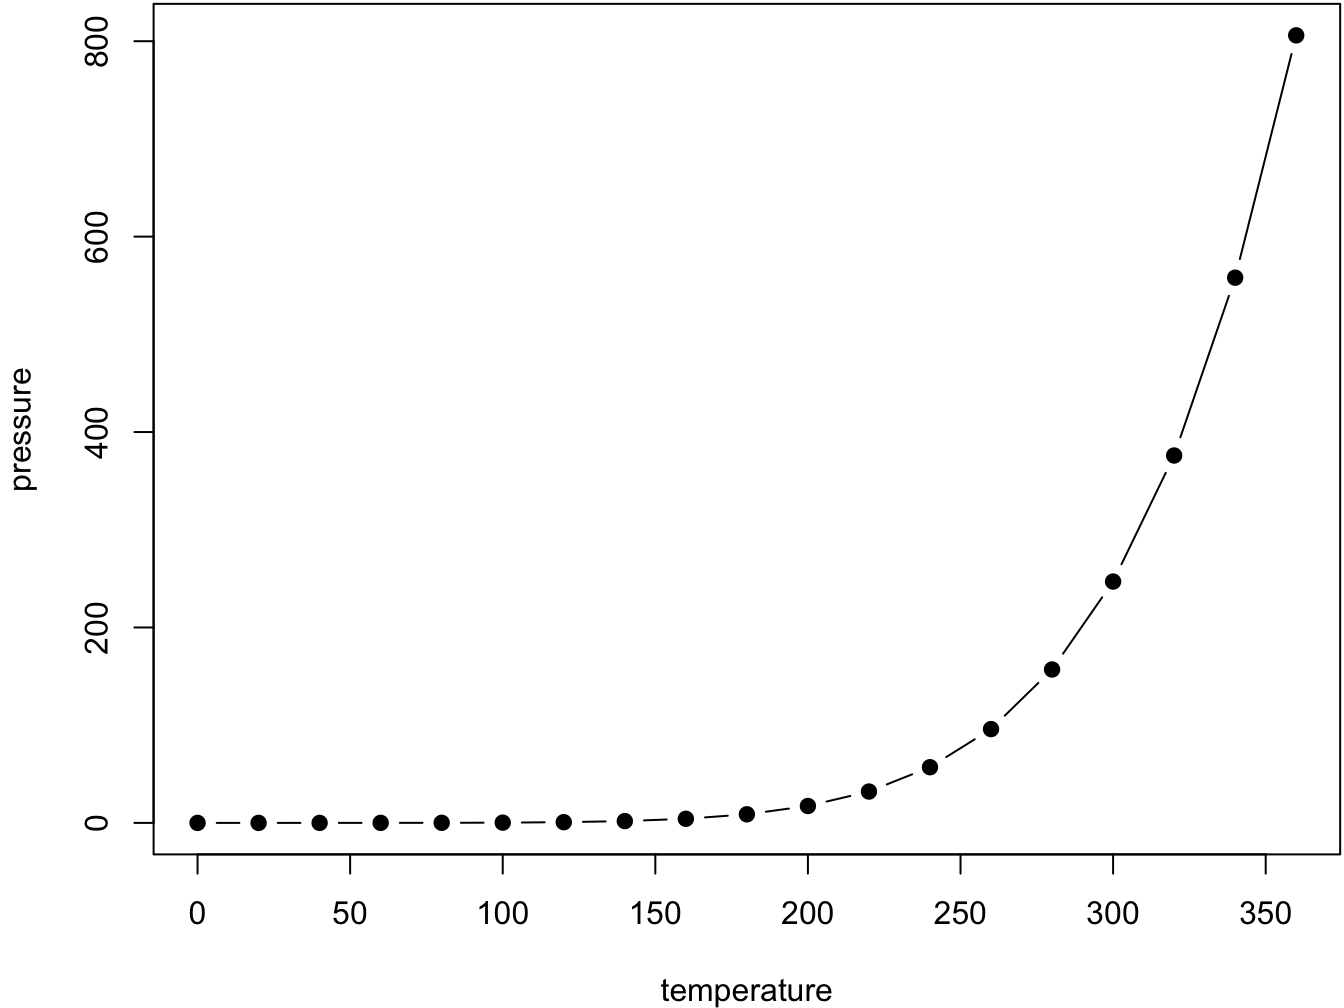
\includegraphics[width=0.8\linewidth]{bookdown-demo_files/figure-latex/nice-fig-1} 

}

\caption{Here is a nice figure!}\label{fig:nice-fig}
\end{figure}

Reference a figure by its code chunk label with the \texttt{fig:}
prefix, e.g., see Figure \ref{fig:nice-fig}. Similarly, you can
reference tables generated from \texttt{knitr::kable()}, e.g., see Table
\ref{tab:nice-tab}.

\begin{Shaded}
\begin{Highlighting}[]
\NormalTok{knitr}\OperatorTok{::}\KeywordTok{kable}\NormalTok{(}
  \KeywordTok{head}\NormalTok{(iris, }\DecValTok{20}\NormalTok{), }\DataTypeTok{caption =} \StringTok{'Here is a nice table!'}\NormalTok{,}
  \DataTypeTok{booktabs =} \OtherTok{TRUE}
\NormalTok{)}
\end{Highlighting}
\end{Shaded}

\begin{table}

\caption{\label{tab:nice-tab}Here is a nice table!}
\centering
\begin{tabular}[t]{rrrrl}
\toprule
Sepal.Length & Sepal.Width & Petal.Length & Petal.Width & Species\\
\midrule
5.1 & 3.5 & 1.4 & 0.2 & setosa\\
4.9 & 3.0 & 1.4 & 0.2 & setosa\\
4.7 & 3.2 & 1.3 & 0.2 & setosa\\
4.6 & 3.1 & 1.5 & 0.2 & setosa\\
5.0 & 3.6 & 1.4 & 0.2 & setosa\\
\addlinespace
5.4 & 3.9 & 1.7 & 0.4 & setosa\\
4.6 & 3.4 & 1.4 & 0.3 & setosa\\
5.0 & 3.4 & 1.5 & 0.2 & setosa\\
4.4 & 2.9 & 1.4 & 0.2 & setosa\\
4.9 & 3.1 & 1.5 & 0.1 & setosa\\
\addlinespace
5.4 & 3.7 & 1.5 & 0.2 & setosa\\
4.8 & 3.4 & 1.6 & 0.2 & setosa\\
4.8 & 3.0 & 1.4 & 0.1 & setosa\\
4.3 & 3.0 & 1.1 & 0.1 & setosa\\
5.8 & 4.0 & 1.2 & 0.2 & setosa\\
\addlinespace
5.7 & 4.4 & 1.5 & 0.4 & setosa\\
5.4 & 3.9 & 1.3 & 0.4 & setosa\\
5.1 & 3.5 & 1.4 & 0.3 & setosa\\
5.7 & 3.8 & 1.7 & 0.3 & setosa\\
5.1 & 3.8 & 1.5 & 0.3 & setosa\\
\bottomrule
\end{tabular}
\end{table}

You can write citations, too. For example, we are using the
\textbf{bookdown} package \citep{R-bookdown} in this sample book, which
was built on top of R Markdown and \textbf{knitr} \citep{xie2015}.

\hypertarget{starting-out-with-r-and-rstudio}{%
\chapter{Starting Out with R and
RStudio}\label{starting-out-with-r-and-rstudio}}

\hypertarget{introduction-and-tools-r-rstudio-and-r-markdown}{%
\subsubsection{Introduction and Tools (R, RStudio, and R
Markdown)}\label{introduction-and-tools-r-rstudio-and-r-markdown}}

\hypertarget{install-r-on-your-computer}{%
\subsubsection{Install R on your
computer}\label{install-r-on-your-computer}}

\hypertarget{install-rstudio}{%
\subsubsection{Install RStudio}\label{install-rstudio}}

\hypertarget{access-datacamp-online}{%
\subsubsection{Access DataCamp online}\label{access-datacamp-online}}

\hypertarget{datacamp-for-rstudio-ide-part-1}{%
\subsubsection{DataCamp for RStudio IDE (Part
1)}\label{datacamp-for-rstudio-ide-part-1}}

\hypertarget{datacamp-for-rstudio-ide-part-2}{%
\subsubsection{DataCamp for RStudio IDE (Part
2)}\label{datacamp-for-rstudio-ide-part-2}}

\hypertarget{access-rstudio-cloud}{%
\subsubsection{Access RStudio cloud}\label{access-rstudio-cloud}}

\hypertarget{r-basics-e-book}{%
\subsubsection{R basics E-book}\label{r-basics-e-book}}

 Use the e-book Rbasics by Chester Ismay

\url{https://ismayc.github.io/rbasics-book/}

\hypertarget{rstudio-tips-document}{%
\subsubsection{RStudio tips document}\label{rstudio-tips-document}}

\hypertarget{importing-your-data}{%
\chapter{Importing Your Data}\label{importing-your-data}}

\hypertarget{lots-of-options-learn-rio}{%
\subsubsection{Lots of options -- learn
rio}\label{lots-of-options-learn-rio}}

\hypertarget{install-rio}{%
\subsubsection{Install rio}\label{install-rio}}

\hypertarget{practice-loading-data-from-multiple-file-types}{%
\subsubsection{Practice loading data from multiple file
types}\label{practice-loading-data-from-multiple-file-types}}

\hypertarget{practice-saving-as-csv-rds-xls-xlsx}{%
\subsubsection{Practice saving as csv, rds, xls,
xlsx}\label{practice-saving-as-csv-rds-xls-xlsx}}

\hypertarget{datacamp-courses-on-import-part-1}{%
\subsubsection{DataCamp Courses on Import (Part
1)}\label{datacamp-courses-on-import-part-1}}

\hypertarget{data-camp-course-on-import-part-2}{%
\subsubsection{Data Camp Course on Import (Part
2)}\label{data-camp-course-on-import-part-2}}

\hypertarget{modern-dive-chapter-1}{%
\subsubsection{Modern Dive Chapter 1}\label{modern-dive-chapter-1}}

\hypertarget{modern-dive-chapter-2}{%
\subsubsection{Modern Dive Chapter 2}\label{modern-dive-chapter-2}}

\hypertarget{chapter-challenges}{%
\subsubsection{Chapter Challenges}\label{chapter-challenges}}

\hypertarget{data-collection}{%
\chapter{Data Collection}\label{data-collection}}

Some \emph{significant} applications are demonstrated in this chapter.

\hypertarget{best-practices-for-data-in-spreadsheets}{%
\subsubsection{Best practices for data in
spreadsheets}\label{best-practices-for-data-in-spreadsheets}}

\url{https://peerj.com/preprints/3183/}

\hypertarget{google-forms-and-googlesheets}{%
\subsubsection{Google Forms and
GoogleSheets}\label{google-forms-and-googlesheets}}

\hypertarget{surveymonkey-data}{%
\subsubsection{SurveyMonkey data}\label{surveymonkey-data}}

\hypertarget{phi-data-redcap-and-redcapr-package}{%
\subsubsection{PHI data -- REDCap and redcapr
package}\label{phi-data-redcap-and-redcapr-package}}

\hypertarget{issues-with-phi-laptops-memory-sticks-cloud-github}{%
\subsubsection{Issues with PHI -- laptops, memory sticks, cloud,
github}\label{issues-with-phi-laptops-memory-sticks-cloud-github}}

\hypertarget{phi-solutions---private-github-mbox-deidentifying-phi-with-charlatan-package-in-r-link-to-phi-that-is-secure}{%
\subsubsection{PHI solutions - private github, M+Box, deidentifying PHI
with charlatan package in R, link to PHI that is
secure}\label{phi-solutions---private-github-mbox-deidentifying-phi-with-charlatan-package-in-r-link-to-phi-that-is-secure}}

\hypertarget{other-sources-of-data}{%
\subsubsection{Other sources of data}\label{other-sources-of-data}}

\hypertarget{surveys-redcap-and-surveymonkey}{%
\paragraph{Surveys -- REDCap and
SurveyMonkey}\label{surveys-redcap-and-surveymonkey}}

\hypertarget{data-direct}{%
\paragraph{Data Direct}\label{data-direct}}

\hypertarget{data-warehouse}{%
\paragraph{Data Warehouse}\label{data-warehouse}}

\hypertarget{checking-validating-and-exploring-your-data}{%
\chapter{Checking, Validating, And Exploring your
Data}\label{checking-validating-and-exploring-your-data}}

\hypertarget{cleaning-names-with-janitor-package-to-snake_case}{%
\subsubsection{Cleaning -- names with janitor package to
snake\_case}\label{cleaning-names-with-janitor-package-to-snake_case}}

\hypertarget{a-few-words-about-tidyverse-style}{%
\paragraph{A few words about tidyverse
style}\label{a-few-words-about-tidyverse-style}}

\hypertarget{finding-missing-data-naniar-and-visdat-packages}{%
\subsubsection{Finding Missing data -- naniar and visdat
packages}\label{finding-missing-data-naniar-and-visdat-packages}}

\hypertarget{validating-data-validate-package}{%
\subsubsection{Validating data -- validate
package}\label{validating-data-validate-package}}

\hypertarget{evaluating-str-glimpse}{%
\subsubsection{Evaluating -- str,
glimpse}\label{evaluating-str-glimpse}}

\hypertarget{exploring--skimr-package}{%
\subsubsection{Exploring- skimr
package}\label{exploring--skimr-package}}

\hypertarget{histograms}{%
\subsubsection{Histograms}\label{histograms}}

\hypertarget{correlations-ggally-extension-of-ggplot2-and-corrr-package}{%
\subsubsection{Correlations -- ggally extension of ggplot2, and corrr
package}\label{correlations-ggally-extension-of-ggplot2-and-corrr-package}}

\hypertarget{data-types}{%
\chapter{Data Types}\label{data-types}}

\hypertarget{numeric---integer-double}{%
\subsubsection{Numeric - Integer,
double}\label{numeric---integer-double}}

\hypertarget{strings-with-the-stringr-package}{%
\subsubsection{Strings with the stringr
package}\label{strings-with-the-stringr-package}}

\hypertarget{rebus-package-and-regex}{%
\paragraph{Rebus package and regex}\label{rebus-package-and-regex}}

\hypertarget{datacamp-strings-course}{%
\paragraph{DataCamp strings course}\label{datacamp-strings-course}}

\hypertarget{factors-with-the-forcats-package}{%
\subsubsection{Factors with the forcats
package}\label{factors-with-the-forcats-package}}

\hypertarget{httpspeerj.compreprints3163}{%
\paragraph{\texorpdfstring{\url{https://peerj.com/preprints/3163/}}{https://peerj.com/preprints/3163/}}\label{httpspeerj.compreprints3163}}

\hypertarget{dates-with-the-lubridate-package}{%
\subsubsection{Dates with the lubridate
package}\label{dates-with-the-lubridate-package}}

\hypertarget{datacamp-dates-and-times-course}{%
\paragraph{DataCamp dates and times
course}\label{datacamp-dates-and-times-course}}

\hypertarget{data-wrangling-with-tidyr-and-dplyr}{%
\chapter{Data Wrangling with Tidyr and
Dplyr}\label{data-wrangling-with-tidyr-and-dplyr}}

\hypertarget{what-is-tidy-data}{%
\subsubsection{What is Tidy Data?}\label{what-is-tidy-data}}

\hypertarget{datacamp-tidyr-course}{%
\subsubsection{DataCamp Tidyr course}\label{datacamp-tidyr-course}}

\hypertarget{try-tidying-new-data---challenges}{%
\paragraph{Try Tidying New Data -
Challenges}\label{try-tidying-new-data---challenges}}

\hypertarget{what-is-data-wrangling}{%
\subsubsection{What is Data Wrangling?}\label{what-is-data-wrangling}}

\hypertarget{datacamp-dplyr-wrangling-course}{%
\subsubsection{DataCamp Dplyr wrangling
course}\label{datacamp-dplyr-wrangling-course}}

\hypertarget{try-wrangling-new-data---challenges}{%
\paragraph{Try Wrangling New Data -
Challenges}\label{try-wrangling-new-data---challenges}}

\hypertarget{general-principles-of-tidying-and-wrangling}{%
\paragraph{General Principles of Tidying And
Wrangling}\label{general-principles-of-tidying-and-wrangling}}

\url{https://peerj.com/preprints/3180/}

\hypertarget{datacamp-dplyr-joins-course}{%
\subsubsection{DataCamp Dplyr joins
course}\label{datacamp-dplyr-joins-course}}

\hypertarget{try-joining-new-data---challenges}{%
\paragraph{Try Joining New Data -
Challenges}\label{try-joining-new-data---challenges}}

\hypertarget{graphic-summaries-for-a-single-variable-with-ggplot}{%
\chapter{Graphic Summaries for a Single Variable with
ggplot}\label{graphic-summaries-for-a-single-variable-with-ggplot}}

\hypertarget{datacamp-ggplot-1-course}{%
\subsubsection{DataCamp ggplot 1
course}\label{datacamp-ggplot-1-course}}

\hypertarget{histograms-1}{%
\subsubsection{Histograms}\label{histograms-1}}

\hypertarget{histogram-challenges}{%
\paragraph{Histogram Challenges}\label{histogram-challenges}}

\hypertarget{boxplot}{%
\subsubsection{Boxplot}\label{boxplot}}

\hypertarget{boxplot-challenges}{%
\paragraph{Boxplot Challenges}\label{boxplot-challenges}}

\hypertarget{violin-plot}{%
\subsubsection{Violin plot}\label{violin-plot}}

\hypertarget{violin-plot-challenges}{%
\paragraph{Violin Plot Challenges}\label{violin-plot-challenges}}

\hypertarget{graphic-summaries-for-a-single-variable-with-ggplot-1}{%
\chapter{Graphic Summaries for a Single Variable with
ggplot}\label{graphic-summaries-for-a-single-variable-with-ggplot-1}}

\hypertarget{datacamp-ggplot-1-course-1}{%
\subsubsection{DataCamp ggplot 1
course}\label{datacamp-ggplot-1-course-1}}

\hypertarget{histograms-2}{%
\subsubsection{Histograms}\label{histograms-2}}

\hypertarget{histogram-challenges-1}{%
\paragraph{Histogram Challenges}\label{histogram-challenges-1}}

\hypertarget{boxplot-1}{%
\subsubsection{Boxplot}\label{boxplot-1}}

\hypertarget{boxplot-challenges-1}{%
\paragraph{Boxplot Challenges}\label{boxplot-challenges-1}}

\hypertarget{violin-plot-1}{%
\subsubsection{Violin plot}\label{violin-plot-1}}

\hypertarget{violin-plot-challenges-1}{%
\paragraph{Violin Plot Challenges}\label{violin-plot-challenges-1}}

\hypertarget{graphic-summaries-for-two-or-more-variables-ggplot2}{%
\chapter{Graphic Summaries for Two or More Variables --
ggplot2}\label{graphic-summaries-for-two-or-more-variables-ggplot2}}

\hypertarget{data-camp-ggplot-course-2}{%
\subsubsection{Data Camp ggplot course
2}\label{data-camp-ggplot-course-2}}

\hypertarget{scatter-plots}{%
\subsubsection{Scatter plots}\label{scatter-plots}}

\hypertarget{mosaic-plots}{%
\subsubsection{Mosaic plots}\label{mosaic-plots}}

\hypertarget{corrr-package}{%
\subsubsection{Corrr package}\label{corrr-package}}

\hypertarget{correlation-matrix}{%
\subsubsection{Correlation matrix}\label{correlation-matrix}}

\hypertarget{descriptive-data-for-two-or-more-variables}{%
\chapter{Descriptive Data for Two or More
Variables}\label{descriptive-data-for-two-or-more-variables}}

\hypertarget{table}{%
\subsubsection{Table}\label{table}}

\hypertarget{janitor-crosstab-tabyl}{%
\subsubsection{Janitor crosstab tabyl}\label{janitor-crosstab-tabyl}}

\hypertarget{presenting-your-results-in-a-report-with-rmarkdown}{%
\chapter{Presenting your Results in a report with
RMarkdown}\label{presenting-your-results-in-a-report-with-rmarkdown}}

\hypertarget{datacamp-rmarkdown-course}{%
\subsubsection{DataCamp Rmarkdown
Course}\label{datacamp-rmarkdown-course}}

\hypertarget{practice-with-data-from-chapter-8---html}{%
\subsubsection{Practice with data from Chapter 8 -
HTML}\label{practice-with-data-from-chapter-8---html}}

\hypertarget{practice-with-data-from-chapter-9---word}{%
\subsubsection{Practice with data from Chapter 9 -
Word}\label{practice-with-data-from-chapter-9---word}}

\hypertarget{practice-with-data-from-chapter-10---ppt}{%
\subsubsection{Practice with data from Chapter 10 -
PPT}\label{practice-with-data-from-chapter-10---ppt}}

\hypertarget{reproducibility-in-your-research}{%
\chapter{Reproducibility in Your
Research}\label{reproducibility-in-your-research}}

\hypertarget{collaborating-with-past-you-and-future-you}{%
\subsubsection{Collaborating with Past You and Future
You}\label{collaborating-with-past-you-and-future-you}}

\hypertarget{general-references}{%
\paragraph{General references}\label{general-references}}

\hypertarget{httpspeerj.compreprints3192}{%
\subparagraph{\texorpdfstring{\url{https://peerj.com/preprints/3192/}}{https://peerj.com/preprints/3192/}}\label{httpspeerj.compreprints3192}}

\hypertarget{httpspeerj.compreprints3139}{%
\subparagraph{\texorpdfstring{\url{https://peerj.com/preprints/3139/}}{https://peerj.com/preprints/3139/}}\label{httpspeerj.compreprints3139}}

\hypertarget{datacamp-github-course}{%
\subsubsection{DataCamp GitHub Course}\label{datacamp-github-course}}

\hypertarget{the-problem-of-versions-and-updated-packages}{%
\subsubsection{The problem of versions and updated
packages}\label{the-problem-of-versions-and-updated-packages}}

\hypertarget{solutions}{%
\paragraph{Solutions}\label{solutions}}

\hypertarget{packrat}{%
\subparagraph{Packrat}\label{packrat}}

\hypertarget{microsoft-r-checkpoint}{%
\subparagraph{Microsoft R checkpoinT}\label{microsoft-r-checkpoint}}

\hypertarget{rocker-docker-containers}{%
\subparagraph{Rocker (docker)
containers}\label{rocker-docker-containers}}

\hypertarget{r-projects}{%
\subsubsection{R Projects}\label{r-projects}}

\hypertarget{rstudio-on-projects}{%
\subsubsection{RStudio on Projects}\label{rstudio-on-projects}}

\hypertarget{multiple-scripts-and-organization-of-projects}{%
\paragraph{Multiple scripts and organization of
projects}\label{multiple-scripts-and-organization-of-projects}}

\hypertarget{version-control}{%
\paragraph{Version control}\label{version-control}}

\hypertarget{httpspeerj.compreprints3159}{%
\subparagraph{\texorpdfstring{\url{https://peerj.com/preprints/3159/}}{https://peerj.com/preprints/3159/}}\label{httpspeerj.compreprints3159}}

\hypertarget{linear-and-branching-projects-and-use-of-the-drake-package}{%
\subsubsection{Linear and branching projects, and use of the drake
package}\label{linear-and-branching-projects-and-use-of-the-drake-package}}

\hypertarget{statistical-inference}{%
\chapter{Statistical inference}\label{statistical-inference}}

\hypertarget{concepts}{%
\subsubsection{Concepts}\label{concepts}}

\hypertarget{datacamp-stats-courses}{%
\subsubsection{DataCamp Stats courses}\label{datacamp-stats-courses}}

\hypertarget{moderndive-chapters}{%
\subsubsection{ModernDive chapters}\label{moderndive-chapters}}

\hypertarget{infer-package-and-practice}{%
\subsubsection{Infer package and
practice}\label{infer-package-and-practice}}

\hypertarget{study-design}{%
\chapter{Study Design}\label{study-design}}

\hypertarget{hypotheses-null-and-alternative}{%
\subsubsection{Hypotheses -- null and
alternative}\label{hypotheses-null-and-alternative}}

\hypertarget{specific-and-testable}{%
\subsubsection{Specific and testable}\label{specific-and-testable}}

\hypertarget{inclusion-and-exclusion}{%
\subsubsection{Inclusion and exclusion}\label{inclusion-and-exclusion}}

\hypertarget{how-many-eligible-patients-datadirect-query}{%
\subsubsection{How many eligible patients -- DataDirect
query}\label{how-many-eligible-patients-datadirect-query}}

\hypertarget{be-conservative-most-wont-enroll}{%
\subsubsection{Be conservative -- most won't
enroll}\label{be-conservative-most-wont-enroll}}

\hypertarget{sample-size-and-power}{%
\chapter{Sample Size and Power}\label{sample-size-and-power}}

\hypertarget{estimating-measures-in-each-group}{%
\subsubsection{Estimating measures in each
group}\label{estimating-measures-in-each-group}}

\hypertarget{estimating-effect-size}{%
\subsubsection{Estimating effect size}\label{estimating-effect-size}}

\hypertarget{estimating-range-and-sd}{%
\subsubsection{Estimating range and SD}\label{estimating-range-and-sd}}

\hypertarget{power-calc-for-continuous}{%
\subsubsection{Power calc for
continuous}\label{power-calc-for-continuous}}

\hypertarget{power-calc-for-proportion}{%
\subsubsection{Power calc for
proportion}\label{power-calc-for-proportion}}

\hypertarget{sources-of-bias}{%
\chapter{Sources of Bias}\label{sources-of-bias}}

\hypertarget{generalizability-of-studies}{%
\subsubsection{Generalizability of
studies}\label{generalizability-of-studies}}

\hypertarget{bias-in-design}{%
\subsubsection{Bias in design}\label{bias-in-design}}

\hypertarget{recall-bias}{%
\subsubsection{Recall Bias}\label{recall-bias}}

\hypertarget{time-bias}{%
\subsubsection{Time bias}\label{time-bias}}

\hypertarget{ascertainment-bias}{%
\subsubsection{Ascertainment bias}\label{ascertainment-bias}}

\hypertarget{assuming-linearity-on-a-scale}{%
\subsubsection{Assuming linearity on a
scale}\label{assuming-linearity-on-a-scale}}

\hypertarget{study-designs}{%
\chapter{Study Designs}\label{study-designs}}

\hypertarget{cross-sectional}{%
\subsubsection{Cross sectional}\label{cross-sectional}}

\hypertarget{cohort}{%
\subsubsection{Cohort}\label{cohort}}

\hypertarget{retrospective}{%
\subsubsection{Retrospective}\label{retrospective}}

\hypertarget{rarely-prospective-registries-case-series-more-likely}{%
\subsubsection{Rarely prospective -- registries, case series more
likely}\label{rarely-prospective-registries-case-series-more-likely}}

\hypertarget{all-associations}{%
\subsubsection{All Associations}\label{all-associations}}

\hypertarget{causal-inference-requires-randomization}{%
\subsubsection{Causal Inference requires
randomization}\label{causal-inference-requires-randomization}}

\hypertarget{one-variable-single-group}{%
\chapter{One variable, single group}\label{one-variable-single-group}}

\hypertarget{continuous-value-t-test}{%
\subsubsection{Continuous value -- t
test}\label{continuous-value-t-test}}

\hypertarget{challenges-for-single-continuous-outcome}{%
\subsubsection{Challenges for single continuous
outcome}\label{challenges-for-single-continuous-outcome}}

\hypertarget{estimate-single-proportion}{%
\subsubsection{Estimate single
Proportion}\label{estimate-single-proportion}}

\hypertarget{challenges-for-single-proportion}{%
\subsubsection{Challenges for single
proportion}\label{challenges-for-single-proportion}}

\hypertarget{one-variable-two-groups}{%
\chapter{One variable, two groups}\label{one-variable-two-groups}}

\hypertarget{variable-1-is-greater-in-group-a-vs-group-b}{%
\subsubsection{Variable 1 is greater in group A vs group
B}\label{variable-1-is-greater-in-group-a-vs-group-b}}

\hypertarget{test-for-skew-if-not-t-test}{%
\paragraph{Test for skew -- if not, T
test}\label{test-for-skew-if-not-t-test}}

\hypertarget{challenges}{%
\subparagraph{Challenges}\label{challenges}}

\hypertarget{if-yes-wilcoxon-non-parametric}{%
\paragraph{If yes, Wilcoxon, non
parametric}\label{if-yes-wilcoxon-non-parametric}}

\hypertarget{challenges-1}{%
\subparagraph{Challenges}\label{challenges-1}}

\hypertarget{variable-2-proportion-is-greater-in-group-a-vs-group-b}{%
\subsubsection{Variable 2 proportion is greater in group A vs group
B}\label{variable-2-proportion-is-greater-in-group-a-vs-group-b}}

\hypertarget{if-no-rare-cells-chi-square}{%
\paragraph{If no rare cells, chi
square}\label{if-no-rare-cells-chi-square}}

\hypertarget{challenges-2}{%
\subparagraph{Challenges}\label{challenges-2}}

\hypertarget{if-rare-cells-fischer-exact-test}{%
\paragraph{If rare cells, Fischer exact
test}\label{if-rare-cells-fischer-exact-test}}

\hypertarget{challenges-3}{%
\subparagraph{Challenges}\label{challenges-3}}

\hypertarget{one-variable-multiple-groups}{%
\chapter{One variable, Multiple
groups}\label{one-variable-multiple-groups}}

\hypertarget{datacamp}{%
\subsubsection{DataCamp}\label{datacamp}}

\hypertarget{fun-with-anova}{%
\subsubsection{Fun with ANOVA}\label{fun-with-anova}}

\hypertarget{challenges-4}{%
\paragraph{Challenges}\label{challenges-4}}

\hypertarget{consider-regression-if-complicated}{%
\subsubsection{Consider Regression if
complicated}\label{consider-regression-if-complicated}}

\hypertarget{linear-regression}{%
\chapter{Linear Regression}\label{linear-regression}}

\hypertarget{datacamp-course}{%
\subsection{DataCamp Course}\label{datacamp-course}}

\hypertarget{single-outcome-multiple-possible-predictors}{%
\subsubsection{Single outcome, multiple possible
predictors}\label{single-outcome-multiple-possible-predictors}}

\hypertarget{challenges-5}{%
\paragraph{Challenges}\label{challenges-5}}

\hypertarget{one-predictor-at-a-time-multiple-univariate-models-modelr-and-broom-packages}{%
\subsubsection{One predictor at a time -- multiple univariate models --
modelr and broom
packages}\label{one-predictor-at-a-time-multiple-univariate-models-modelr-and-broom-packages}}

\hypertarget{challenges-6}{%
\paragraph{Challenges}\label{challenges-6}}

\hypertarget{choosing-predictors-for-multivariate-modeling-testing-dealing-with-collinearity}{%
\subsubsection{Choosing predictors for multivariate modeling -- testing,
dealing with
collinearity}\label{choosing-predictors-for-multivariate-modeling-testing-dealing-with-collinearity}}

\hypertarget{challenges-7}{%
\paragraph{Challenges}\label{challenges-7}}

\hypertarget{multivariate-modeling}{%
\subsubsection{Multivariate modeling}\label{multivariate-modeling}}

\hypertarget{challenges-8}{%
\paragraph{Challenges}\label{challenges-8}}

\hypertarget{model-fit-checking}{%
\subsubsection{Model fit checking}\label{model-fit-checking}}

\hypertarget{challenges-9}{%
\paragraph{Challenges}\label{challenges-9}}

\hypertarget{presenting-model-results-with-rmarkdown}{%
\subsubsection{presenting model results with
RMarkdown}\label{presenting-model-results-with-rmarkdown}}

\hypertarget{challenges-10}{%
\paragraph{Challenges}\label{challenges-10}}

\hypertarget{sharing-models-with-shiny}{%
\chapter{Sharing Models with Shiny}\label{sharing-models-with-shiny}}

\hypertarget{datacamp-courses-on-shiny}{%
\subsubsection{DataCamp Courses on
Shiny}\label{datacamp-courses-on-shiny}}

\hypertarget{practice-with-model-from-20}{%
\subsubsection{Practice with model from
20}\label{practice-with-model-from-20}}

\hypertarget{logistic-regression}{%
\chapter{Logistic Regression}\label{logistic-regression}}

\hypertarget{concepts-and-or}{%
\subsubsection{Concepts and OR}\label{concepts-and-or}}

\hypertarget{modeling}{%
\subsubsection{Modeling}\label{modeling}}

\hypertarget{estimating-gof}{%
\subsubsection{Estimating GOF}\label{estimating-gof}}

\hypertarget{auroc}{%
\subsubsection{AuROC}\label{auroc}}

\hypertarget{sens-spec-ppv-npv}{%
\subsubsection{Sens Spec PPV NPV}\label{sens-spec-ppv-npv}}

\hypertarget{confusion-matrix}{%
\subsubsection{Confusion Matrix}\label{confusion-matrix}}

\hypertarget{present-results-with-broom-rmarkdown}{%
\subsubsection{Present results with broom,
RMarkdown}\label{present-results-with-broom-rmarkdown}}

\hypertarget{make-user-friendly-model-predictions-with-shiny}{%
\subsubsection{Make user-friendly model predictions with
Shiny}\label{make-user-friendly-model-predictions-with-shiny}}

\hypertarget{meta-analysis}{%
\chapter{Meta-Analysis}\label{meta-analysis}}

\hypertarget{data-search}{%
\subsubsection{Data search}\label{data-search}}

\hypertarget{data-collection-1}{%
\subsubsection{Data collection}\label{data-collection-1}}

\hypertarget{data-exclusion}{%
\subsubsection{Data Exclusion}\label{data-exclusion}}

\hypertarget{data-extraction-and-checking}{%
\subsubsection{Data extraction and
checking}\label{data-extraction-and-checking}}

\hypertarget{using-metafor-package}{%
\subsubsection{Using Metafor package}\label{using-metafor-package}}

\hypertarget{making-figures}{%
\subsubsection{Making Figures}\label{making-figures}}

\hypertarget{writing-up-results-in-rmarkdown}{%
\subsubsection{Writing up results in
RMarkdown}\label{writing-up-results-in-rmarkdown}}

\bibliography{book.bib,packages.bib}


\end{document}
